\section{EINDTOETS · Statistiek}

\begin{missie}
Missie: toon wat je kan. Alle leerplandoelen komen aan bod.
\end{missie}

\textbf{Naam:} \_\_\_\_\_\_\_\_\_\_\_\_\_\_\_\_\_\_\_\_\_\_\_\_\_\_\_\_\_\_ \quad \textbf{Klas:} \_\_\_\_\_\_\_\_\_\_\_\_\_ \quad \textbf{Datum:} \_\_\_\_\_\_\_\_\_\_\_\_\_

\textbf{Hulpmiddelen:} rekentoestel of GeoGebra/Excel, potlood, gom. \quad \textbf{Duur:} ongeveer 60 minuten. \quad \textbf{Totaal:} 60 punten.

\begin{letop}
\textbf{Zo werk je:} schrijf je werkwijze op. Geef bij kansen telkens het model, een schets en een antwoordzin. Rond af op twee decimalen tenzij anders vermeld.
\end{letop}

\textbf{Doelenmatrix: welke vraag test welk doel?}

\breedtes{40/30/30}
\begin{tabular}{lcc}
\hline
Doel & Vragen & Punten \\
\hline
Springplank: populatie, steekproef, variabelen, centrum- en spreidingsmaten & 1 – 5 & 20 \\
LPD 11: representativiteit, selectiebias, steekproefgrootheid en parameter & 6 – 7 & 7 \\
LPD 12: samenhang en causaliteit, onderzoeksopzet & 8 – 10 & 10 \\
LPD 13: normale verdeling als model & 11 – 13 & 11 \\
LPD 14: kansen bij een normale verdeling (ICT) & 14 – 16 & 12 \\
LPD 1 – 4: beschrijven, problemen oplossen, ICT, communiceren & verweven in 3, 5, 14 – 16 & \\
\hline
\end{tabular}

\subsection*{A · Basis: begrippen en kengetallen}

\textbf{Vraag 1 \quad (4 p)} Een kinderopvang met 320 ingeschreven kinderen wil weten hoeveel dagen per week de kinderen naar de opvang gaan. Ze bevraagt de ouders van 50 kinderen. Noteer de populatie, de steekproef, de variabele en het soort variabele, en geef $N$ en $n$. \lijn

\begin{oplossing}
\textbf{Oplossing 1} \quad Populatie: de 320 kinderen van de opvang ($N=320$) (1); steekproef: de 50 bevraagde kinderen ($n=50$) (1); variabele: aantal dagen opvang per week (1); kwantitatief – numeriek, discreet (1).
\end{oplossing}

\textbf{Vraag 2 \quad (3 p)} Aan 36 deelnemers van een ouderavond werd gevraagd hoe tevreden ze zijn.

\breedtes{55/20}
\begin{tabular}{lc}
\hline
antwoord & AF \\
\hline
zeer ontevreden & 2 \\
ontevreden & 4 \\
noch ontevreden, noch tevreden & 6 \\
tevreden & 15 \\
zeer tevreden & 9 \\
\hline
\end{tabular}

Bepaal de modus en de mediaan en verklaar waarom je geen gemiddelde kan berekenen. \lijn

\begin{oplossing}
\textbf{Oplossing 2} \quad Mod = tevreden (15 keer) (1). Cumulatief 2 – 6 – 12 – 27 – 36; het 18de en 19de gegeven zitten in ‘tevreden’: Med = tevreden (1). Het zijn categorisch geordende data (woorden), je kan er niet mee optellen of delen (1).
\end{oplossing}

\textbf{Vraag 3 \quad (4 p)} Het aantal uren vrijwilligerswerk van 8 jongeren in een maand: 6 – 2 – 9 – 4 – 7 – 4 – 3 – 21.

\textbf{a)} Bereken het gemiddelde, de mediaan en de modus. (3 p) \lijn

\textbf{b)} Welke centrummaat geeft het beste beeld van een ‘typische’ jongere? Waarom? (1 p) \lijn

\begin{oplossing}
\textbf{Oplossing 3} \quad Rangschikken: 2 – 3 – 4 – 4 – 6 – 7 – 9 – 21. a) $\overline{x}=\dfrac{56}{8}=7$ uur (1); $\text{Med}=\dfrac{4+6}{2}=5$ uur (1); Mod = 4 uur (1). b) De mediaan (of de modus): het gemiddelde wordt omhooggetrokken door de uitschieter 21 (1).
\end{oplossing}

\textbf{Vraag 4 \quad (5 p)} Gebruik dezelfde data als in vraag 3.

\textbf{a)} Bepaal de variatiebreedte, $Q_1$, $Q_3$ en de interkwartielafstand. (4 p) \lijn

\textbf{b)} Interpreteer de interkwartielafstand in een zin. (1 p) \lijn

\begin{oplossing}
\textbf{Oplossing 4} \quad a) $R=21-2=19$ (1); onderste helft 2 – 3 – 4 – 4: $Q_1=\dfrac{3+4}{2}=3{,}5$ (1); bovenste helft 6 – 7 – 9 – 21: $Q_3=\dfrac{7+9}{2}=8$ (1); $\Delta Q=8-3{,}5=4{,}5$ (1). b) De middelste 50 \% van de jongeren doet vrijwilligerswerk met een verschil van hoogstens 4,5 uur (1).
\end{oplossing}

\textbf{Vraag 5 \quad (4 p)} Vijf collega’s hebben 2 – 3 – 5 – 6 – 9 jaar ervaring. Ze vormen de volledige populatie. Bereken de variantie en de standaardafwijking (2 decimalen). Toon je tussenstappen. \lijn

\begin{oplossing}
\textbf{Oplossing 5} \quad $\mu=\dfrac{25}{5}=5$ (1); afwijkingen $-3$, $-2$, 0, 1, 4; kwadraten 9, 4, 0, 1, 16, som 30 (1); $\sigma^2=\dfrac{30}{5}=6$ jaar² (1); $\sigma=\sqrt{6}\approx 2{,}45$ jaar (1).
\end{oplossing}

\subsection*{B · Steekproef en representativiteit (LPD 11)}

\textbf{Vraag 6 \quad (4 p)} Een gemeente wil weten of de inwoners tevreden zijn over de nieuwe speelpleinen. Ze plaatst een vragenlijst op haar Facebookpagina. Er komen 2\,000 antwoorden binnen.

\textbf{a)} Is dit een representatieve steekproef? Verklaar. (2 p) \lijn

\textbf{b)} Hoe kan de gemeente een representatievere steekproef bekomen? (2 p) \lijn

\begin{oplossing}
\textbf{Oplossing 6} \quad a) Nee (1): enkel wie de pagina volgt en wil antwoorden reageert (zelfselectie, onderdekking van wie geen Facebook gebruikt); een groot aantal antwoorden maakt de steekproef niet representatief (1). b) Door aselecte trekking uit de volledige bevolkingslijst (1) en door ervoor te zorgen dat de geselecteerde mensen ook effectief antwoorden, bv. via brief of telefoon (1).
\end{oplossing}

\textbf{Vraag 7 \quad (3 p)} Een steekproef van 100 jongeren geeft een gemiddelde slaapduur van 7,6 uur met een standaardafwijking van 1,0 uur.

\textbf{a)} Noteer deze twee getallen met de juiste symbolen en zeg welke parameters ze schatten. (2 p) \lijn

\textbf{b)} Waarom hoeft het gemiddelde van alle jongeren niet precies 7,6 uur te zijn? (1 p) \lijn

\begin{oplossing}
\textbf{Oplossing 7} \quad a) $\overline{x}=7{,}6$ uur schat $\mu$; $s=1{,}0$ uur schat $\sigma$ (2). b) Steekproefvariabiliteit: een andere steekproef geeft door toeval een ander gemiddelde (1).
\end{oplossing}

\subsection*{C · Samenhang en causaliteit (LPD 12)}

\textbf{Vraag 8 \quad (4 p)} Uit onderzoek blijkt: ‘Kinderen uit gezinnen met veel boeken thuis lezen beter.’

\textbf{a)} Is dit samenhang of causaliteit? (1 p) \lijn

\textbf{b)} Geef een verborgen variabele die beide kan verklaren. (2 p) \lijn

\textbf{c)} Geef een omgekeerde verklaring. (1 p) \lijn

\begin{oplossing}
\textbf{Oplossing 8} \quad a) Samenhang; er is geen bewijs van causaliteit (1). b) Bv. het opleidingsniveau of de leesgewoonte van de ouders (1): zij kopen meer boeken én stimuleren het lezen (1). c) Kinderen die graag lezen, krijgen meer boeken cadeau (1).
\end{oplossing}

\textbf{Vraag 9 \quad (4 p)} Een woonzorgcentrum wil onderzoeken of een dagelijkse wandeling de stemming van bewoners verbetert. Beschrijf een experiment met testgroep en controlegroep en leg uit waarom de indeling door loting gebeurt. \lijn

\begin{oplossing}
\textbf{Oplossing 9} \quad Testgroep: wandelt dagelijks (1); controlegroep: geen wandeling, gewone zorg (1); bewoners worden door loting verdeeld (1) zodat de groepen vergelijkbaar zijn en verborgen variabelen (bv. gezondheid) gelijk verdeeld zijn (1); stemming wordt in beide groepen op dezelfde manier gemeten.
\end{oplossing}

\textbf{Vraag 10 \quad (2 p)} Koppel aan elke uitspraak de verklaring \textbf{V} (verborgen variabele), \textbf{O} (omgekeerde causaliteit): \textbf{a)} Hoe meer ijsjes verkocht, hoe meer zonnebrand. \_\_ \quad \textbf{b)} Wie veel slaapmiddelen neemt, slaapt slechter. \_\_

\begin{oplossing}
\textbf{Oplossing 10} \quad a) V (warm weer) (1) \quad b) O (wie slecht slaapt, neemt slaapmiddelen) (1).
\end{oplossing}

\subsection*{D · De normale verdeling als model (LPD 13)}

\textbf{Vraag 11 \quad (4 p)} Twee histogrammen met bijhorende kengetallen.

\begin{center}
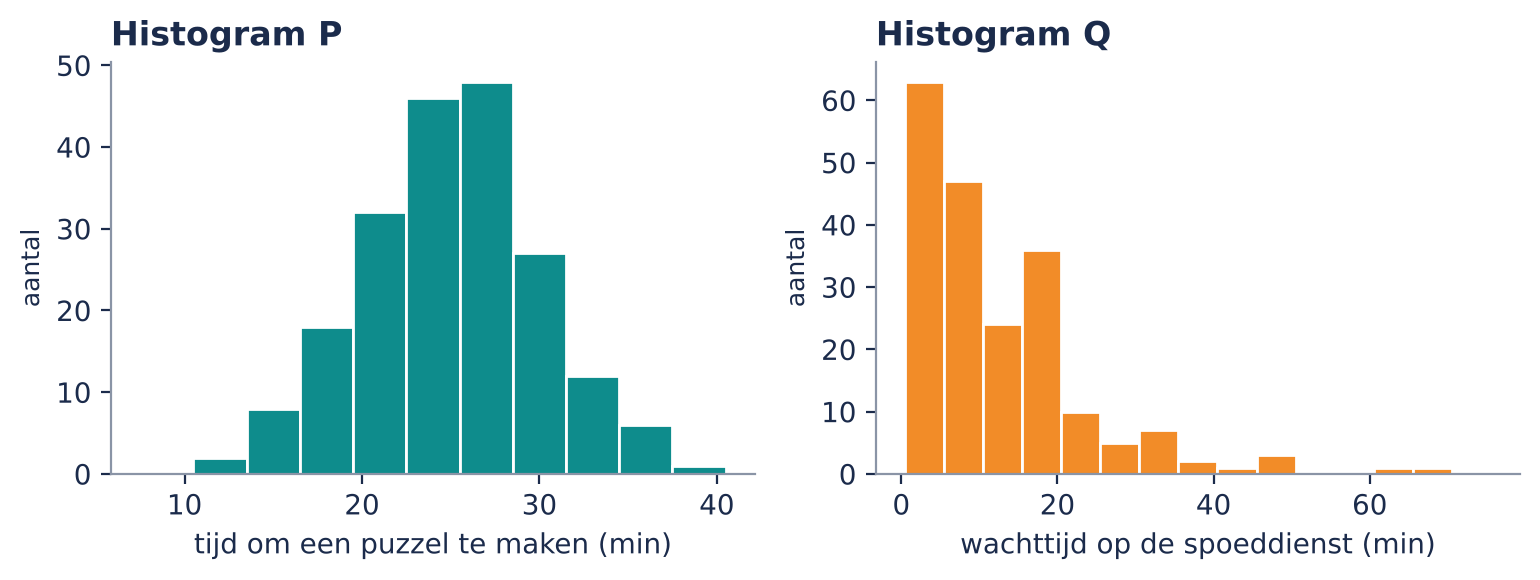
\includegraphics[width=0.95\textwidth]{figuren/toets_histogrammen.png}
\end{center}

\breedtes{35/30/35}
\begin{tabular}{lcc}
\hline
 & Histogram P & Histogram Q \\
\hline
gemiddelde & 25,0 min & 12,6 min \\
mediaan & 25,0 min & 10,0 min \\
standaardafwijking & 5,0 min & 11,1 min \\
\hline
\end{tabular}

Voor welk histogram is een normaal model geschikt? Verklaar je keuze voor beide histogrammen met de grafiek én de kengetallen. \lijn

\begin{oplossing}
\textbf{Oplossing 11} \quad P: ja (1): klokvormig, symmetrisch, één top (1), gemiddelde = mediaan (25). Q: nee (1): scheef naar rechts, met een lange staart, gemiddelde (12,6) duidelijk groter dan de mediaan (10) (1).
\end{oplossing}

\textbf{Vraag 12 \quad (4 p)} De reactietijd van leerlingen is bij benadering normaal verdeeld. Een steekproef van 200 leerlingen geeft $\overline{x}=0{,}45$ s en $s=0{,}06$ s.

\textbf{a)} Noteer het model $N(\mu,\sigma)$. (1 p) \lijn

\textbf{b)} Tussen welke waarden ligt ongeveer 95 \% van de reactietijden? (2 p) \lijn

\textbf{c)} Een andere groep heeft hetzelfde gemiddelde maar een standaardafwijking van 0,10 s. Hoe verschilt de Gausskromme van die groep? (1 p) \lijn

\begin{oplossing}
\textbf{Oplossing 12} \quad a) $N(0{,}45;\,0{,}06)$ (1). b) $\mu\pm 2\sigma$: $0{,}45\pm 0{,}12$, dus tussen 0,33 s en 0,57 s (2). c) Dezelfde top (zelfde $\mu$), maar de kromme is breder en lager (1).
\end{oplossing}

\textbf{Vraag 13 \quad (3 p)} Een normaal verdeelde variabele heeft zijn top bij $x=120$ en buigpunten bij $x=105$ en $x=135$. Bepaal $\mu$ en $\sigma$ en bereken hoeveel procent van de waarden groter is dan 150. \lijn

\begin{oplossing}
\textbf{Oplossing 13} \quad $\mu=120$ (1); $\sigma=135-120=15$ (1); $150=\mu+2\sigma$, dus ongeveer $\dfrac{100-95}{2}=2{,}5$ \% is groter dan 150 (1).
\end{oplossing}

\subsection*{E · Kansen bij de normale verdeling (LPD 14) en problemen oplossen}

\textbf{Vraag 14 \quad (4 p)} De wachttijd bij het ophalen van kinderen is normaal verdeeld met $\mu=12$ min en $\sigma=3$ min. Bereken met ICT de kans dat een ouder:

\textbf{a)} langer dan 15 minuten wacht; (2 p) \lijn

\textbf{b)} tussen 9 en 18 minuten wacht. (2 p) \lijn

\begin{oplossing}
\textbf{Oplossing 14} \quad a) $X\sim N(12;\,3)$; $P(X>15)\approx 0{,}1587$ (2): ongeveer 15,9 \% (denk ook aan de regel: 15 = $\mu+\sigma$, dus $\approx 16$ \%). b) $P(9<X<18)\approx 0{,}8186$ (2): ongeveer 81,9 \%.
\end{oplossing}

\textbf{Vraag 15 \quad (4 p)} Een kinderverzorger plant 20 minuten voor elke maaltijd. De duur van een maaltijd is normaal verdeeld met $\mu=16$ min en $\sigma=3$ min.

\textbf{a)} Wat is de kans dat een maaltijd uitloopt (langer dan 20 minuten duurt)? Schrijf het model, een schets en een antwoordzin. (3 p) \lijn

\textbf{b)} Hoeveel van 40 maaltijden lopen naar verwachting uit? (1 p) \lijn

\begin{oplossing}
\textbf{Oplossing 15} \quad a) $X\sim N(16;\,3)$ (1); schets met rechterstaart gearceerd (1); $P(X>20)\approx 0{,}0912$: een maaltijd loopt in ongeveer 9,1 \% van de gevallen uit (1). b) $40\cdot 0{,}0912\approx 3{,}6$, dus ongeveer 4 maaltijden (1).
\end{oplossing}

\textbf{Vraag 16 \quad (4 p)} Twee klassen maken dezelfde toets (op 100). Beide hebben een gemiddelde van 72 punten; de punten zijn normaal verdeeld. Klas A heeft een standaardafwijking van 4 punten, klas B van 12 punten.

\textbf{a)} Bereken voor beide klassen de kans dat een leerling meer dan 80 punten haalt. (2 p) \lijn

\textbf{b)} Vergelijk beide klassen in twee zinnen met centrum- en spreidingsmaten en je resultaten uit a). (2 p) \lijn

\begin{oplossing}
\textbf{Oplossing 16} \quad a) Klas A: $P(X>80)\approx 0{,}0228$ (1). Klas B: $P(X>80)\approx 0{,}2525$ (1). b) Beide klassen hebben hetzelfde gemiddelde (72); in klas B is de spreiding veel groter ($s=12$ tegenover $4$) (1). Daardoor haalt in klas B ongeveer een kwart van de leerlingen meer dan 80, in klas A slechts 2,3 \%; klas B heeft dus meer uitblinkers, maar ook meer zwakke resultaten (1).
\end{oplossing}

\begin{doel}
\textbf{Mijn score:} \_\_\_\_ / 60 \quad \textbf{Behaald vanaf 36 / 60 (60 \%).}

Per onderdeel: Basis \_\_ / 20 \quad LPD 11 \_\_ / 7 \quad LPD 12 \_\_ / 10 \quad LPD 13 \_\_ / 11 \quad LPD 14 \_\_ / 12
\end{doel}
